\documentclass[10.5pt]{jsarticle}
%\usepackage{otf} %Windows上ではコメントアウトしてね
\usepackage{amsmath, amssymb}
\usepackage[dvipdfmx]{graphics,xcolor}
\usepackage{tikz}
\usepackage[framemethod=tikz]{mdframed}
\usepackage{type1cm}
\usepackage{graphicx}
\usepackage{float}
\usepackage{here}
\usepackage{fancyhdr}
\usepackage{lscape} %ページ全体を用いた横向き画像使用時に使用
\usepackage{tabularx}

%マージン設定
%横
\setlength{\textwidth}{165truemm}
\setlength{\hoffset}{-1truein}
\setlength{\oddsidemargin}{25truemm}
%縦
\setlength{\textheight}{257truemm}
\setlength{\voffset}{-1truein}
\setlength{\topmargin}{10truemm}
\setlength{\headheight}{5truemm}
\setlength{\headsep}{5truemm}

%ページ番号設定
\pagestyle{fancy}
\fancyhead[RE]{}
\fancyhead[RO]{\thepage}
\fancyhead[LE]{\thepage}
\fancyhead[LO]{}
\cfoot{}
\renewcommand{\headrulewidth}{0pt}

%図表番号設定
%「図4.4.1」みたいにしたかったらsectionをsubsectionに変える
\makeatletter
\renewcommand{\figurename}{図}
\renewcommand{\thefigure}{\thesection.\arabic{figure}}
\@addtoreset{figure}{section}
\makeatother
\makeatletter
\renewcommand{\tablename}{表}
\renewcommand{\thetable}{\thesection.\arabic{table}}
\@addtoreset{table}{section}
\makeatother

%箇条書き表示設定
\renewcommand{\labelenumi}{(\arabic{enumi})}%第1階層
\renewcommand{\labelenumii}{(\roman{enumii})}%第2階層

%タイトル設定
\title{「通信ネットワーク」 キーポイント}
\author{}
\date{\vspace{-10mm}3年 後期}

%「jlisting.sty」が必要
\usepackage{listings,jlisting}
\def\lstlistingname{リスト}	%キャプションの設定
\lstset{%
language={Java},
basicstyle={\small},%
identifierstyle={\small},%
commentstyle={\small\itshape},%
keywordstyle={\small\bfseries},%
ndkeywordstyle={\small},%
stringstyle={\small\ttfamily},
frame={tb},
breaklines=true,
columns=[l]{fullflexible},%
numbers=left,%
xrightmargin=0zw,%
xleftmargin=3zw,%
numberstyle={\scriptsize},%
stepnumber=1,
numbersep=1zw,%
lineskip=-0.5ex%
}

\begin{document}

%タイトルの出力
\maketitle
\thispagestyle{fancy}

\section{ネットワークを構成する2つの基本要素}
ネットワークは,端末および中心の処理系を示すノードとノード間の通信線路を示すリンクによって構成される.ネットワーク図においてはノードは円で描かれ,リンクはそれらを直線で結ぶように描かれる.

\section{*LAN,MAN,WANの正式名称と適用領域}
\begin{enumerate}
	\item{LAN : Local-Area Network}\\
		施設内などに設けられた広がりが数百メートル以内のネットワーク.
	\item{MAN : Metropolitan-Area Network}\\
		都市内の通信に用いられる広がりが数十キロメートル以内のネットワーク.
	\item{WAN : Wide-Area Network}\\
		都市間およびそれ以上の長距離を結ぶネットワーク.広がりは数十キロメートル以上.
\end{enumerate}

\section{*ネットワークの各種トポロジー}
\begin{enumerate}
\item{メッシュ : Mesh}\\
ノード同士が規則なく相互に通信しあうネットワーク.全てノードが相互に通信しあう場合を特にフルメッシュ(Full-Mesh)という.
通信には無数の経路が考えられるため障害耐性は高いが,線路が多く敷設費用が高い.
\item{スター : Star}\\
1つのノードを中心ノードとし,そのノードからその他のノードへ放射状にリンクが伸びているネットワーク.
中心ノードは基地局と呼ばれる.
管理のしやすさと費用の面から,一般的な加入者線はこの形態をとる.
ただし中心ノードで障害が発生した場合に全てのネットワークがダウンするため,障害耐性は低い.
\item{リング : Ring}\\
リンクが円を描くように隣接するノード間にのみ存在するネットワーク.
1つの線路で障害が発生した場合にも逆方向から通信が可能であるが,2箇所以上障害が発生した場合通信が一切できなくなる.
\item{バス : Bus}\\
中心にバス線があり,全てのノードはそのバス線と直接リンクで結ばれている.
送信した信号が全ての端末で受信される.
全てのノードがバス線を共有するため,信号の衝突による干渉が発生しないような工夫が必要になる.
\item{トリー : Tree}\\
ルートノードから枝分かれする様に伸びていくネットワーク.
CATVのシステムやUSBのような1対多通信が主になる場合に使われる.
\end{enumerate}
以上のネットワークを図示すると,図\ref{topology}のようになる.
\begin{figure}[h]
	\centering
	\begin{minipage}{0.25\hsize}
		\centering
		\includegraphics[width=0.8\hsize]{files/topology_mesh.ai}\\
		(a)メッシュ
	\end{minipage}
	\begin{minipage}{0.25\hsize}
		\centering
		\includegraphics[width=0.8\hsize]{files/topology_star.ai}\\
		(b)スター
	\end{minipage}
	\begin{minipage}{0.25\hsize}
		\centering
		\includegraphics[width=0.8\hsize]{files/topology_ring.ai}\\
		(c)リング
	\end{minipage}
	\begin{minipage}{0.35\hsize}
		\centering
		\includegraphics[width=0.8\hsize]{files/topology_bus.ai}\\
		(d)バス
	\end{minipage}
	\begin{minipage}{0.35\hsize}
		\centering
		\includegraphics[width=0.8\hsize]{files/topology_tree.ai}\\
		(e)トリー
	\end{minipage}
	\caption{各種トポロジ}\label{topology}
\end{figure}

\section{*メッシュ網,スター網,リング網におけるノード数と伝送路数の関係}
全てのノード数を$n$とする.
\begin{enumerate}
\item{メッシュ網}\\
ここではフルメッシュについて考えるものとする.
フルメッシュである場合,全てのノード同士が1つのリンクによって結ばれるため,伝送路数は全てのノードから2つのノードを取り出す組み合わせに等しく,\underline{${}_nC_2$}である.
\item{スター網}\\
中心ノードを除く$n-1$個のノードが各々1つずつ中心ノードとのリンクを持つ.
よって伝送路数は\underline{$n-1$}である.
\item{リング網}\\
全てのノードを頂点として多角形を描くようにリンクが存在するため,伝送路数は$n$角形の辺の数に等しく,\underline{$n$}である.
\end{enumerate}

\section{経路切替え型ネットワークと媒体共有型ネットワークの相違点および具体例}


\section{電話ネットワークにおいて2線式および4線式通信路の違いと使い分けられている理由}


\section{呼量[単位:アーラン(Erlang)]の算出法}
呼量とは,ネットワークを構成する設備の中を流れる信号の量(トラヒック量)を呼量と呼ぶ.
呼量は,一定時間$T$において$n$回生起した呼の保留時間(通話時間)をそれぞれ,$t_1, t_2, \cdots , t_n$とすると,
\[\displaystyle a = \frac{\displaystyle \sum_{i=1}^n t_i}{T}\]
と定義される.

\section{*回線交換方式とパケット交換方式の原理および前者に比べた時の後者の長所・短所(p12~)}
\begin{description}
 \item[回線交換方式]\mbox{}\\ 
	    回線交換では通信が開始されると送信端末と受信端末がひとつの物理的な回線で接続され通信の終了まで維持される。
 \item[パケット交換方式]\mbox{}\\
	    伝送路を介した隣接交換機間の通信を一つの単位とし、それらの最適な組み合わせをパケットごとに選ぶことによって、動的な回路が実現される。
 \item[パケット交換方式の長所]\mbox{}\\
・高い信頼性(交換機機関で誤り制御と再送処理ができるため)\\・異種サービスへの対応(パケットという共通の信号形式のため異種サービスの端末をネットワークへ直接接続可能なため)\\・ネットワークの有効利用(ネットワークを専有しないため)\\・情報量に応じた課金(パケットという単位を使っているため)
\item[パケット交換方式の短所]\mbox{}\\
・信号からパケットへの変換やその逆変換で必要な信号処理回路、パケットを蓄積するためのメモリなど回線交換では使わない高度なハードウェアが必要になる\\・ネットワーク内での蓄積や信号処理によって生じる遅延や、ネットワークを経て届くパケットの中で最も遅いものに合わせて処理が行われることによる遅延など、回路交換に存在しない遅延がある。\\・ルーティング、フロー制御、蓄積などの信号処理が多くなるので回線交換に比べて通信の高速化が困難である。
\end{description}

\section{*データ通信ネットワークにおける集中型と分散型の違いと具体例(p17~)}
\begin{description}
 \item[集中型ネットワーク]\mbox{}\\ 
	    大容量の情報を高速で処理可能なコンピュータ(ホスト)がセンターにあり、データの入出力と必要最小限の処理が可能なコンピュータ(端末)を各所に設けて、ホストと端末とを個別にスター型トポロジーで接続する。使用例は座席予約システムや登録システム、超高速計算機の共同利用システムなど。
 \item[分散型ネットワーク]\mbox{}\\
	    大量のデータを蓄積するとともに、その内容に関する外部からの要求に対して反応を返すことができるコンピュータ(サーバ)とユーザが個々に必要とする処理能力とデータ蓄積能力もつコンピュータ(クライアント)とがネットワークを介して自由に接続されている。さらに各コンピュータが対等に通信できる。使用例はインターネットや、LAN。
\end{description}


\section{*OSI参照モデルの各層の名称}
OSI参照モデルを図\ref{osi_refmodel}に示す.名称は
\begin{figure}[h]
	\centering
	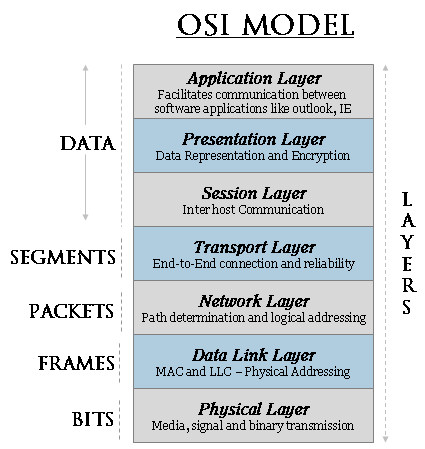
\includegraphics[width=7.5cm]{files/protocols_osi_model.ai}
	\caption{OSI参照モデル}\label{osi_refmodel}
\end{figure}



\section{媒体共有型ネットワークを分類したときの3つの形式とそれぞれの特徴}
\begin{table}[H]
	\centering
	\caption{媒体共有型ネットワークの分類} \label{media-sharing-network}
	\begin{tabularx}{0.9\hsize}{|l|X|} 
		\hline
		\multicolumn{1}{|c|}{\textbf{種類}}&\multicolumn{1}{c|}{\textbf{概要}}\\\hline\hline
		ランダムアクセス型&各端末が,他端末との調整をすることなくそれぞれの判断で信号を送出する.
							できる限り衝突を減らすため,送出の前と後に伝送媒体をモニターする必要がある.\\\hline
		トークンパッシング型&端末間で信号送出権を巡回させ,できる限り公平に信号を送出できるようにする.
							そのために特殊な制御信号(トークン)を用い,これを受信した端末が信号を送出する.\\\hline
		ポーリンング型&端末に信号送出権を与える役割を担う制御局をネットワーク内に設ける.
							制御曲は送出したい信号を保持している端末に順次送出権を割り当てる.\\\hline
	\end{tabularx}
\end{table}


\section{*ランダムアクセス型のプロトコルであるALOHAにおいて,トラヒックとスループットをそれぞれ横軸と縦軸で表したときに得られるカーブの形(略図)そのような形になる定性的理由}
ALOHAにおいて,単位時間あたりの平均$\lambda$回発生するパケットが時間$t$の間に$k$回発生する確率はポアソン分布に従う.
各フレームの持続時間を$T$とすると,全フレームの占める延べ時間は$\lambda T$である.
このときトラヒックは$g=\lambda T$と定義されるから,$\lambda = g/T$と表され,ポアソン分布は次式で与えられることとなる.
\[P(t, k) = \frac{(gt/T)^k}{k!}e^{-gt/T}\]

パケットが有効であることは時間幅$2T$の間に他のパケットが送信されないことであるから,パケットが有効である確率$P$は$t=2T, k=0$として次式で表される.
\[P = P(2T, 0) = e^{-2g}\]
このときスループット$s$はトラヒック$g$と確率$P$の積で与えられる.
\[s = g \times P = ge^{-2g}\]
これをグラフ上に描くと,図\ref{}のように$(g, s) = (0.5, 0.18)$の点で極大値をとることとなる.

\section{ランダムアクセス型のプロトコルであるCSMAの送信アルゴリズムがALOHAから改良されている点およびその効果}
ALOHAは,送出したパケットが正しく受信されなかったことを検出した後,ランダムに時間を空けてもう一度信号を送出する.
これに対し,CSMA(Carrier Sense Multiple Acces)はパケットを送出する前にネットワークの状況を把握(キャリアセンス)し,
他のパケットが存在したら送出を取りやめる.
他のパケットを検出したときには,ランダムに時間を空けてパケットを送出するように試みる.

\section{*CSMA/CDの送信制御アルゴリズム}



\section{MACアドレスとは}



\section{*FDDIにおける信号制御用フレームの名称と信号制御アルゴリズム}



\section{FDDIでのネットワーク障害復旧のための手法(略図)}



\section{*ATM方式でのセルおよびその中のペイロード部分のサイズ}



\section{ATMセルのペイロード長を国際標準化で決める際2つの分野から出された相反する要求}



\section{*符号誤り制御における垂直・水平パリティ方式の原理.垂直パリティ方式と比べたときの改良点}

垂直パリティ方式の複数のビット列を図7-2のようにそれぞれ垂直方向に配置し、それらを水平方向に並べた後、末尾に各ビット列と同じ長さを持つ別のビット列を一つ付加する。この2次元に配置されたビットを水平方向に見て、各行における”1”の個数が偶数(または奇数)になるように付加ビット列の中の各ビット(水平パリティコード)を決める。

垂直パリティ方式の一つのビット列長より短いバースト誤りであれば検出することができる。

\section{*CRC符号の求め方}

8ビットのデータ信号 10010101 を送受信する場合を考える。この信号に対応する多項式P(X)は

\begin{equation}
  P(X) = X^7 + X^4 + X^2 + 1
\end{equation}
である。ここで生成多項式G(X)を
\begin{equation}
 G(X) = X^6 + X^4 + X^2 + 1
\end{equation}
とし、G(X)の最高次数6を次数とする項 $X^6$ をP(X)に掛けて新たな多項式
\begin{equation}
 X^6 P(X) = X^{13} + X^{10} + X^8 + X^6
\end{equation}
を作り、これをG(X)で割る。演算の結果割り算の余りが
\begin{equation}
 R(X) = X^5 + X^4
\end{equation}
であるから、送信信号に対応する多項式は
\begin{equation}
 T(X) = X^6 P(X) + R(X) = X^{13} + X^{10} + X^8 + X^6 + X^5 + X^4
\end{equation}

とある。送信信号はこの多項式に対応してビット列10010101110000となる。このうち末尾の110000がCRC符号である。

\section{*ハミング距離と符号誤り検出,符号誤り訂正の関係}



\section{畳み込み符号とビタビ復号アルゴリズムの概要}



\section{TCP/IP階層モデルとOSI参照モデルの対応関係}



\section{*TCPおよびIPの正式名称とそれぞれの役割}
TCPはTransmission Control Protocolの略であり,IPはInternet Protocolの略である.前者は受信側へ欠落や順不同のないパケットを届けるためのものであり,
後者は複数のネットワークを相互接続してそれらの間にIPパケットを伝達するためのものである.


\section{*IPアドレスおよびサブネットマスク}
IPアドレスはIPにおける識別番号であり,IPv4なら32ビット,IPv6なら128ビットの2進数で表される.
その役割は手紙の輸送における住所と似ている.


\section{*IPv6のねらい}



\section{*(サブ)ネットワークアドレスとブルードキャストアドレス}



\section{*グローバルIPアドレスとプライベートIPアドレスの意味と,それらが使い分けられている理由}



\section{ルーティングテーブルを用いたルータの動作}



\section{ARPおよびDNSの役割}



\section{*ドメイン名,IPアドレス,MACアドレスについて,それぞれの意味・目的および相互の変換手法}



\section{コネクション型通信とコネクションレス通信の違い}


\section{IP電話サーバの役割}


\section{携帯電話システムにおけるホームメモリの役割}


\section{*携帯電話システムにおけるセルサイズの大小と利点・問題点}
携帯電話の通信において一つの基地局が受け持つ通信領域をセルという。セルの半径が大きいと、その内部に存在する携帯端末のトラヒックを請け負うため、多くの周波数資源が必要になる。それに対して、セルの半径を小さくすると、相互に干渉しあわない距離にあるセル間で、同一の周波数をもちいて、周波数を再利用する方式がとれる(周波数利用効率の向上)。また送信電力の低減も可能である。しかしセルを小さくすることで、基地局やハンドオーバの増大が発生する。ちなみに、このようなセルを基本としたネットワークによる携帯電話方式を「セルラー」という。

\section{*ハンドオーバとは}
通信中に移動端末が隣接するセル業界を横切った場合に、回線を基地局で切り替えて通信を継続させることをハンドオーバという。ハンドオーバ時に通信品質の低下(瞬断など)が生じないようにすることが重要である。

\section{ISM帯とは}


\section{無線LANにおけるインフラモードとアドホックモードの違い}


\section{隠れ端末問題およびさらされ端末問題とは(略図)}


\section{隠れ端末問題およびさらされ端末問題を解決するための手法}


\section{リアクティブ型ルーティングの手法(略図)}


\end{document}
